% !TeX document-id = {6ded82bc-a22c-4503-a090-6b5ed60b2b6b}
% !TeX program = lualatex
% !TeX TXS-program:bibliography = txs:///bibtex

\documentclass[
xcolor=dvipsnames,
aspectratio=169,
9pt,
%handout,
]{beamer}

\definecolor{uniSblue}{RGB}{0,65,145}
\definecolor{uniSlightblue}{RGB}{0,190,255}
\definecolor{uniSgrey}{RGB}{62, 68, 76}
\definecolor{uniSyellow}{RGB}{255, 213, 0}

% colors not covered by CD but still useful
\definecolor{uniSred}{RGB}{230, 0, 50}
\definecolor{uniSgreen}{RGB}{0, 200, 50} 

%\usetheme{Luebeck}
\usetheme{boxes}
%\usecolortheme{beaver} %rot
\usecolortheme{seagull} %grau

%\usepackage[utf8]{inputenc}
\usepackage[T1]{fontenc}

\usepackage{fontspec}
\defaultfontfeatures{Ligatures=TeX}
%\usepackage[]{unicode-math} 
%\unimathsetup{math-style=TeX}
%\setmainfont[SmallCapsFeatures={LetterSpace=6}, Numbers={Proportional,OldStyle}, Ligatures=TeX]{Univers for UniS 55 Roman Rg}
%\setmonofont[Scale=0.9]{Hack}
%\setmainfont[SmallCapsFeatures={LetterSpace=6}, Numbers={Proportional,OldStyle}]{Minion Pro}
%\setmainfont[LetterSpace=3, Numbers={Proportional,OldStyle}, Ligatures=TeX]{Myriad Pro}
\defaultfontfeatures{Mapping=tex-text}
%

\usepackage{tikz, pgfplots}

\usepackage[ngerman, english]{babel}% Silbentrennung

%do not ovelap with footer line
\addtobeamertemplate{footnote}{}{\vspace{2.5ex}}

%footnotes without numbering with \blankfootnote{}
\let\svthefootnote\thefootnote
\textheight 1in
\newcommand\blankfootnote[1]{%
	\let\thefootnote\relax\footnotetext{\tiny #1}%
	\let\thefootnote\svthefootnote%
}



%item color setzen
\setbeamercolor{itemize item}{fg=uniSlightblue}
\setbeamercolor{itemize subitem}{fg=uniSlightblue}


\setbeamercolor{block title}{bg=uniSlightblue,fg=white}
\setbeamercolor{block body}{bg=uniSlightblue!10,fg=black}

\setbeamercolor*{structure}{bg=uniSlightblue,fg=uniSlightblue}

\setbeamercolor*{palette primary}{use=structure,fg=uniSlightblue,bg=structure.fg}
\setbeamercolor*{palette secondary}{use=structure,fg=uniSlightblue,bg=structure.fg!75}
\setbeamercolor*{palette tertiary}{use=structure,fg=white,bg=black}
\setbeamercolor*{palette quaternary}{fg=white,bg=black}

\setbeamercolor{section in toc}{fg=black,bg=white}
\setbeamercolor{alerted text}{use=structure,fg=structure.fg!50!black!80!black}

\setbeamercolor{titlelike}{parent=palette primary,fg=structure.fg!50!black}
\setbeamercolor{frametitle}{bg=white,fg=uniSgrey}

\setbeamercolor*{titlelike}{parent=palette primary}


%\setbeamercovered{transparent}

\setbeamertemplate{navigation symbols}{}%remove navigation symbols
\setbeamertemplate{itemize items}[circle]



% http://tex.stackexchange.com/questions/55806/tikzpicture-in-beamer/55827#55827
  \tikzset{
    invisible/.style={opacity=0},
    visible on/.style={alt=#1{}{invisible}},
    alt/.code args={<#1>#2#3}{%
      \alt<#1>{\pgfkeysalso{#2}}{\pgfkeysalso{#3}} % \pgfkeysalso doesn't change the path
    },
  }
  \tikzset{onslide/.code args={<#1>#2}{%
  \only<#1>{\pgfkeysalso{#2}} % \pgfkeysalso doesn't change the path
}}




\newcommand{\partitle}[1]{\textcolor{uniSlightblue}{\textbf{#1}}\\ \smallskip}

% argument #1: any options
\newenvironment{customlegend}[1][]{%
	\begingroup
	% inits/clears the lists (which might be populated from previous
	% axes):
	\csname pgfplots@init@cleared@structures\endcsname
	\pgfplotsset{#1}%
}{%
	% draws the legend:
	\csname pgfplots@createlegend\endcsname
	\endgroup
}%

\pgfplotsset{compat=newest}


% makes \addlegendimage available (typically only available within an
% axis environment):
\def\addlegendimage{\csname pgfplots@addlegendimage\endcsname}
\def\addlegendentry{\csname pgfplots@addlegendentry\endcsname}




\usepackage{bm}

\usepackage{wasysym}

% possibly needed TikZ libraries
\usetikzlibrary{calc,fit, positioning, patterns, decorations.pathmorphing, decorations.markings, shapes, shapes.geometric, shapes.callouts, arrows.meta, shadings, trees, chains, 3d, shadows}

% Toleranzen mit tikz darstellen
%\input{tikzTolerances}

% camera shape. 
% Draw with \camera{(xshift, yshift)}{rotationDeg}{Label}
\def\camera#1#2#3{
	\begin{scope}[shift={#1}, rotate=#2, fill=white]
		\draw [fill=black](0,0) -- (0.5,0.75) -- (-0.5,0.75) -- cycle;
		\node [fill=white,thick, minimum height=1cm, draw] at (0,0){#3};
	\end{scope}
}

% TikZ blocks

% mechanical:
\tikzstyle{spring}=[thick,decorate,decoration={zigzag,pre length=0.3cm,post length=0.3cm,segment length=6}]
\tikzstyle{damper}=[thick,decoration={markings,  
	mark connection node=dmp,
	mark=at position 0.5 with 
	{
		\node (dmp) [thick,inner sep=0pt,transform shape,rotate=-90,minimum width=15pt,minimum height=3pt,draw=none] {};
		\draw [thick] ($(dmp.north east)+(2pt,0)$) -- (dmp.south east) -- (dmp.south west) -- ($(dmp.north west)+(2pt,0)$);
		\draw [thick] ($(dmp.north)+(0,-5pt)$) -- ($(dmp.north)+(0,5pt)$);
	}
}, decorate]
\tikzstyle{ground}=[fill,pattern=north east lines,draw=none,minimum width=0.75cm,minimum height=0.3cm]

% electrical and control theory:
\tikzstyle{block} = [draw=black, fill=white, rectangle, text centered, minimum height=3em, minimum width=3em]
\tikzstyle{sum} = [draw, circle, node distance=1cm]
\tikzstyle{input} = [coordinate]
\tikzstyle{output} = [coordinate]
\tikzstyle{new} = [fill=uniSlightblue!20]
\tikzstyle{gain} = [regular polygon, regular polygon sides=3,
draw, fill=white, text width=1em,
inner sep=1mm, outer sep=0mm,
shape border rotate=-90]

\tikzset{cross/.style={cross out, draw, minimum size=2*(#1-\pgflinewidth), inner sep=0pt, outer sep=0pt, line width=4pt}}

% more conveient arrow heads
\tikzset{>={Latex[width=2mm,length=2mm]}}

% line width global definition for unique layout
\tikzset{every picture/.style={line width=0.6pt}}


% Fancy node streching from http://tex.stackexchange.com/a/124507
% Examples:
%
%\node[right=of |(A)(B)(D)]          {Z};
%
%\node[left=of |(A)(B), ultra thick] {Y};
%\node[left=of |(C)(D), minimum width=50pt]          (X) {X};
%
%\node[span vertical=(A)(B), above=of -X] {y};
%
%\node[below=of -(A)(B)(C)(D)] {0};
\makeatletter
\def\pgfutil@firstofmany#1#2\pgf@stop{#1}
\def\pgfutil@secondofmany#1#2\pgf@stop{#2}
\def\tikz@lib@place@of@#1#2#3{%
	\def\pgf@tempa{fit bounding box}%
	\edef\pgf@temp{\expandafter\pgfutil@firstofmany#2\pgf@stop}
	\if\pgf@temp(%
	\tikz@lib@place@fit@scan{#2}{0}%
	\else\if\pgf@temp|
	\expandafter\tikz@lib@place@fit@scan\expandafter{\pgfutil@secondofmany#2\pgf@stop}{1}%
	\else\ifx\pgf@temp\tikz@activebar
	\expandafter\tikz@lib@place@fit@scan\expandafter{\pgfutil@secondofmany#2\pgf@stop}{1}%
	\else\if\pgf@temp-
	\expandafter\tikz@lib@place@fit@scan\expandafter{\pgfutil@secondofmany#2\pgf@stop}{2}%
	\else\if\pgf@temp+
	\expandafter\tikz@lib@place@fit@scan\expandafter{\pgfutil@secondofmany#2\pgf@stop}{3}%
	\else
	\def\pgf@tempa{#2}%
	\fi
	\fi
	\fi
	\fi
	\fi
	\expandafter\tikz@scan@one@point\expandafter\tikz@lib@place@remember\expandafter(\pgf@tempa)%
	\iftikz@shapeborder%
	% Ok, this is relative to a border.
	\iftikz@lib@ignore@size%
	\edef\tikz@node@at{\noexpand\pgfpointanchor{\tikz@shapeborder@name}{center}}%
	\def\tikz@anchor{center}%
	\else%
	\edef\tikz@node@at{\noexpand\pgfpointanchor{\tikz@shapeborder@name}{#3}}%
	\fi%
	\fi%
	\edef\tikz@lib@place@nums{#1}%
}
\def\tikz@lib@place@fit@scan#1#2{
	\pgf@xb=-16000pt\relax%
	\pgf@xa=16000pt\relax%
	\pgf@yb=-16000pt\relax%
	\pgf@ya=16000pt\relax%
	\if\pgfutil@firstofmany#1\pgf@stop(%
	\tikz@lib@fit@scan#1\pgf@stop%
	\else
	\tikz@lib@fit@scan(#1)\pgf@stop
	\fi
	\ifdim\pgf@xa>\pgf@xa
	% shouldn't happen
	\else
	\expandafter\def\csname pgf@sh@ns@fit bounding box\endcsname{rectangle}%
	\expandafter\edef\csname pgf@sh@np@fit bounding box\endcsname{%
		\def\noexpand\southwest{\noexpand\pgfqpoint{\the\pgf@xa}{\the\pgf@ya}}%
		\def\noexpand\northeast{\noexpand\pgfqpoint{\the\pgf@xb}{\the\pgf@yb}}%
	}%
	\expandafter\def\csname pgf@sh@nt@fit bounding box\endcsname{{1}{0}{0}{1}{0pt}{0pt}}%
	\expandafter\def\csname pgf@sh@pi@fit bounding box\endcsname{\pgfpictureid}%
	\ifcase#2\relax
	\or % 1 = vertical
	\pgf@y=\pgf@yb%
	\advance\pgf@y by-\pgf@ya%
	\edef\pgf@marshal{\noexpand\tikzset{minimum height={\the\pgf@y-2*(\noexpand\pgfkeysvalueof{/pgf/outer ysep})}}}%
	\pgf@marshal
	\or % 2 = horizontal
	\pgf@x=\pgf@xb%
	\advance\pgf@x by-\pgf@xa%
	\edef\pgf@marshal{\noexpand\tikzset{minimum width={\the\pgf@x-2*(\noexpand\pgfkeysvalueof{/pgf/outer xsep})}}}%
	\pgf@marshal
	\or % 3 = both directions
	\pgf@y=\pgf@yb%
	\advance\pgf@y by-\pgf@ya%
	\pgf@x=\pgf@xb%
	\advance\pgf@x by-\pgf@xa%
	\edef\pgf@marshal{\noexpand\tikzset{minimum height={\the\pgf@y-2*(\noexpand\pgfkeysvalueof{/pgf/outer ysep})},minimum width={\the\pgf@x-2*(\noexpand\pgfkeysvalueof{/pgf/outer xsep})}}}%
	\pgf@marshal
	\fi
	\fi
}
\tikzset{
	fit bounding box/.code={\tikz@lib@place@fit@scan{#1}{0}},
	span vertical/.code={\tikz@lib@place@fit@scan{#1}{1}},
	span horizontal/.code={\tikz@lib@place@fit@scan{#1}{2}},
	span/.code={\tikz@lib@place@fit@scan{#1}{3}}}

\makeatother


%pgfplots settings
\pgfplotsset{
	compat = newest,
	%tick label style = {font=\sansmath\sffamily},
	%every axis label = {font=\sansmath\sffamily},
	%legend style = {font=\sansmath\sffamily},
	%label style = {font=\sansmath\sffamily},
	grid=major,
	every axis plot/.append style={thick},
}

%% 3D drawings

% 3D drawings axes mapping onto 2D image projection
\tikzset{math3d/.style= {x={(1cm, 0cm)}, y={(.353cm,.353cm)}, z={(0cm,1cm)}}}

% other 3D drawing views
\tikzstyle{isometric}=[x={(0.710cm,-0.410cm)},y={(0cm,0.820cm)},z={(-0.710cm,-0.410cm)}]
\tikzstyle{dimetric} =[x={(0.935cm,-0.118cm)},y={(0cm,0.943cm)},z={(-0.354cm,-0.312cm)}]
\tikzstyle{dimetric2}=[x={(0.935cm,-0.118cm)},z={(0cm,0.943cm)},y={(+0.354cm,+0.312cm)}]
\tikzstyle{dimetric3} =[y={(0.935cm,-0.118cm)},z={(0cm,0.943cm)},x={(-0.354cm,-0.312cm)}]
\tikzstyle{trimetric}=[x={(0.926cm,-0.207cm)},y={(0cm,0.837cm)},z={(-0.378cm,-0.507cm)}]

%Call: \tikzblock{Breite}{Höhe}{Tiefe}{Zusätze}
\newcommand{\tikzblock}[4]{\filldraw[#4] (0,0,0) rectangle (#1,0,#2);
	\filldraw[fill=black!5, #4] (0,0,#2)--(0,#3,#2) --(#1,#3,#2) --(#1,0,#2) -- cycle;
	\filldraw[fill=black!20, #4] (#1,0,0) -- (#1,0,#2)-- (#1,#3,#2) -- (#1,#3,0) -- cycle;}

\newcommand{\colouredtikzblock}[4]{\filldraw[fill=uniSlightblue!50, draw=uniSlightblue!50, #4] (0,0,0) rectangle (#1,0,#2);
	\filldraw[fill=uniSlightblue!30, draw=uniSlightblue!50,#4] (0,0,#2)--(0,#3,#2) --(#1,#3,#2) --(#1,0,#2) -- cycle;
	\filldraw[fill=uniSlightblue, draw=uniSlightblue!50,#4] (#1,0,0) -- (#1,0,#2)-- (#1,#3,#2) -- (#1,#3,0) -- cycle;}

%Aufruf: \tikzplaneXZ{x-Dimension}{z-Dimension}{Zusätze}
\newcommand{\tikzplaneXZ}[3]{\filldraw[#3] (0,0,0) -- (#1,0,0) -- (#1,0,#2) -- (0,0,#2) -- cycle;}

%Aufruf: \tikzplaneXZ{x-Dimension}{y-Dimension}{Zusätze}
\newcommand{\tikzplaneXY}[3]{\filldraw[fill=black!5,#3] (0,0,0) -- (#1,0,0) -- (#1,#2,0) -- (0,#2,0) -- cycle;}

%Aufruf: \tikzplaneYZ{y-Dimension}{z-Dimension}{Zusätze}
\newcommand{\tikzplaneYZ}[3]{\filldraw[fill=black!20,#3] (0,0,0) -- (0,#1,0) -- (0,#1,#2) -- (0,0,#2) -- cycle;}

% Pandocs Tightlist command
\providecommand{\tightlist}{%
	\setlength{\itemsep}{0pt}\setlength{\parskip}{0pt}}



%external TikZ, pgf for faster compiling and exportable figures
%\usetikzlibrary{external}
%\tikzset{external/mode=graphics if exists}
%\tikzexternalize[prefix=..img/tikz/]
%%\tikzset{external/force remake}

%matlab2tikz options
\newlength\fheight 
\newlength\fwidth 
\setlength\fheight{3cm} 
\setlength\fwidth{12cm}

\newcommand{\fillhalfrb}[3]{%
	\begin{scope}[on background layer]
		\fill[fill=#2] (#1.north west)--(#1.south west)--(#1.north east)--cycle;
		\fill[fill=#3] (#1.north east)--(#1.south east)--(#1.south west)--cycle;
	\end{scope}	
}

%Strechable skip to get contents a the bottom of slides
\newcommand{\btVFill}{\vskip0pt plus 1filll}

\makeatletter
\newcommand*{\defeq}{\mathrel{\rlap{%
			\raisebox{0.3ex}{$\m@th\cdot$}}%
		\raisebox{-0.3ex}{$\m@th\cdot$}}%
	=}
\makeatother

\newcommand{\ddiff}{\mathrm{d}}
\newcommand{\R}{\ensuremath{\mathbb{R}}}
\newcommand{\C}{\ensuremath{\mathbb{C}}}

\newcommand{\bmat}[1]{\ensuremath{\begin{bmatrix} #1 \end{bmatrix}}}

\newcommand{\imgsource}[1]{\begin{flushright}
		\textcolor{black!40}{\tiny Source:~#1}	
\end{flushright}}

\newcommand{\follows}{\ensuremath{\Rightarrow}}
\newcommand{\gdw}{\ensuremath{\Leftrightarrow}}

\usetikzlibrary{backgrounds}

%\usepackage{tikz-uml}
\usepackage{multimedia}
\usepackage{media9} 
\graphicspath{{./img/}}

%%TITLE
\defbeamertemplate*{title page}{customized}[1][]
{
	\begin{tikzpicture}[remember picture,overlay]
		\filldraw[uniSgrey!20]([yshift=-40pt]current page.north west) rectangle (current page.south east);
		\node[anchor=north west] 
		at ([yshift=-4pt, xshift=10pt]current page.north west) (logo)
		{\parbox[t]{.19\paperwidth}{\raggedleft%
				\usebeamercolor[fg]{titlegraphic}\inserttitlegraphic}};
		
		\node[anchor= west] 
		at ([xshift=4em, yshift=-20pt]current page.west) (STRimage)
		{
\includegraphics[width=.4\paperwidth]{../img/STR}};
		
		\node[fill=uniSgrey!80!black, circle, minimum size=18em, inner sep=0.3em, align=left, text width=14em] at ([xshift=-5cm, yshift=-0.5cm]current page.east) {
		\begin{minipage}[][5cm][c]{5cm}	
			{\raggedleft\scriptsize \textcolor{white}{\insertinstitute}}\\\vfill
			{\raggedleft\usebeamerfont{title}\textcolor{white}{\normalsize\textbf{\inserttitle}}}\\
			{\raggedleft\usebeamerfont{subtitle}\textcolor{white}{\small\textit{\insertsubtitle}}}\\\vfill
			{\raggedleft\usebeamerfont{date}\textcolor{white}{\footnotesize\insertdate}}
		\end{minipage}
		};
		\node[fill=white, circle, minimum size=2em, inner sep=5pt, align=center, text=uniSgrey, font=\footnotesize\selectfont] at ([xshift=-6em, yshift=-8em]current page.east) {\authorForTitle};
	\end{tikzpicture}	
}

%%TITLE_END



\title[Simulation-based control of Soft Materials with an Industrial Robot]{Simulation-based control of Soft Materials with an Industrial Robot}


\author{F. Jaensch, J. Terfurth, M. Wnuk, Z. Chen, D. Tomzik, Jax, Amy, Sivakumar, Massi}
\newcommand{\authorForTitle}{C. Hinze, F. Jaensch,\\ J. Köhler, B. Maier,\\ S. Shavanez, D. Tomzik,\\ M. Wnuk}
\titlegraphic{
\includegraphics[height=30pt]{LogosUSTUTT_UOA}}
\institute{DFG IRTG GRK2198/1\newline Soft Tissue Robotics}
\date{06 July 2018}


% This is only inserted into the PDF information catalog. Can be left
% out.
\subject{IRTG Project presentation}

\begin{document}
	
	\addtobeamertemplate{frametitle}{}{%
		\begin{tikzpicture}[remember picture,overlay]
		\node[anchor=north east,yshift=3pt,xshift=0pt] at (current page.north east)
		{
\includegraphics[height=0.8cm]{img/LogosUSTUTT_UOA}};
		\end{tikzpicture}}
	
	%{\usebackgroundtemplate{\includegraphics[height=1.0\paperheight]{img/cnc_milling_low.jpg}}
		\begin{frame}
		\titlepage
		\end{frame}%}

\setbeamertemplate{footline}[text line]{%
	\parbox{\linewidth}{\vspace*{-8pt}\insertframenumber\hfill %\insertshortauthor:~
    \insertshorttitle\hfill}}
\setbeamertemplate{navigation symbols}{}

\AtBeginSection[]{
\begin{frame}
\frametitle{Contents}
\tableofcontents[ 
currentsubsection, 
hideothersubsections, 
sectionstyle=show/shaded, 
subsectionstyle=show/shaded, 
] 
%You might wish to add the option [pausesections]
\end{frame}
}

\AtBeginSubsection[]{
	\begin{frame}
	\frametitle{Contents}
	\tableofcontents[ 
	currentsubsection, 
	hideothersubsections, 
	sectionstyle=show/hide, 
	subsectionstyle=show/shaded, 
	] 
	%You might wish to add the option [pausesections]
	\end{frame}
}


%% Build a slide like this and place LaTeX content within
%\begin{frame}{Frame title}
%
%\end{frame}
% ----------------------------------------------------------------------------------------------------------
% ----------------------------------------------------------------------------------------------------------
%\section{Motivation}
%% ----------------------------------------------------------------------------------------------------------
%
%\begin{frame}{What is intelligence?}
%	\begin{tabular}{c p{10cm}}
%		\structure{Definition:} & "...the resultant of the process of \structure{acquiring}, \structure{storing} in memory, \structure{retrieving}, \structure{combining}, \structure{comparing}, and \structure{using} in new contexts \structure{information} and conceptual skills" \\& 		- Lloyd Humphreys
%	\end{tabular}
%	
%		\begin{center}
%		\movie[width=0.5\linewidth,
%		height=0.28125\linewidth,poster,loop]{}{vid/MotivationVid_Challenge_Ape.mov}
%	\end{center}	
%	
%%	\begin{center}	
%%		\includemedia[
%%		height=4.5cm,
%%		keepaspectratio,
%%		activate=pageopen,
%%		addresource=vid/MotivationVid_Challenge_final.MP4,
%%		flashvars={source=vid/MotivationVid_Challenge_final.MP4}
%%		]{}{VPlayer.swf}
%%	\end{center} 
%\end{frame}

% ----------------------------------------------------------------------------------------------------------
%\begin{frame}{Industrial Challenges \& Applications}
%	
%	\begin{center}
%		\movie[width=0.8\linewidth,
%		height=0.45\linewidth,poster]{}{vid/MotivationVid_Industrial.mov}
%	\end{center}
%	
%	
%%	\begin{center}
%%		\includemedia[
%%			width=0.5\linewidth,
%%			height=0.45\linewidth,
%%			activate=pageopen,
%%			addresource=vid/MotivationVid_Industrial.MP4,
%%			flashvars={source=vid/MotivationVid_Industrial.MP4}
%%			]{}{VPlayer.swf}
%%		\end{center} 	
%	
%\end{frame}
%
%\begin{frame}{Medical Challenges \& Applications}
%	\begin{center}
%		\movie[width=0.8\linewidth,
%		height=0.45\linewidth,poster]{}{vid/MotivationVid_Medical.mov}
%	\end{center}	
%	
%%	\includemedia[
%%		width=0.8\linewidth,
%%		height=0.45\linewidth,
%%		activate=pageopen,
%%		addresource=vid/MotivationVid_Medical.MP4,
%%		flashvars={source=vid/MotivationVid_Medical.MP4}
%%		]{}{VPlayer.swf}
%\end{frame}



% ----------------------------------------------------------------------------------------------------------
\section{Setup description}
\begin{frame}{Motivation}
	\begin{columns}
		\begin{column}{0.4\textwidth}
			\begin{itemize}
				\item Say why our task is important
				\item ...
			\end{itemize}
		\end{column}
		\begin{column}{0.6\textwidth}
			\begin{center}
				\begin{figure}
					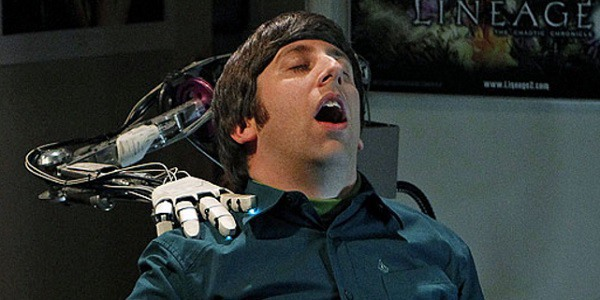
\includegraphics[width=1\textwidth]{img/Wolowitz.jpg}
					\caption{Robotic teleoperation in an everyday scenario. Picture taken from the SitCom ``The Big Bang Theory''}
				\end{figure}
			\end{center}
		\end{column}
	\end{columns}
\end{frame}

\begin{frame}{Goal}
	\begin{columns}
		\begin{column}{0.4\textwidth}
			\begin{itemize}
				\item Define goal set for the demonstrator week here
				\item ...
			\end{itemize}
		\end{column}
		\begin{column}{0.6\textwidth}
			\begin{center}
				\begin{figure}
					\resizebox{0.6\columnwidth}{!}{
					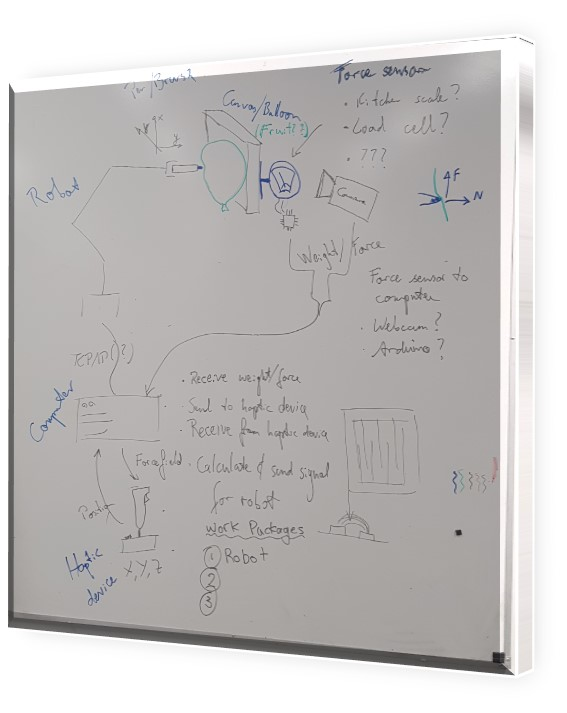
\includegraphics[width=1\textwidth]{img/ConceptDrawing.jpg}
					}
					\caption{Original concept for the 2019 summer school demonstrator}
				\end{figure}
			\end{center}
		\end{column}
	\end{columns}
\end{frame}

\begin{frame}{Problem formulation}
	\begin{columns}
		\begin{column}{0.4\textwidth}
			\begin{itemize}
				\item Here goes the description of the involved problems
				\item Force feedback from soft tissue
				\item control for the system
				\item sensor
				\item communication and interfaces
				\item ...
			\end{itemize}
		\end{column}
		\begin{column}{0.6\textwidth}
			\begin{center}
				\begin{figure}
					\resizebox{0.8\columnwidth}{!}{
						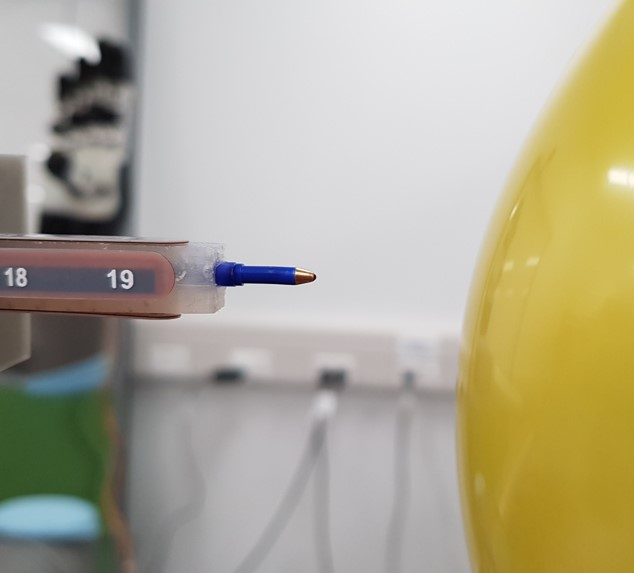
\includegraphics[width=1\textwidth]{img/ProblemDescription_BallandPen.jpg}
					}
					\caption{Balloon and pen during a drawing task. The pointy tip of the pen threatens to burst the balloon.}
				\end{figure}
			\end{center}
		\end{column}
	\end{columns}
\end{frame}


%-------------------------------------------------------------------------------

\section{Concept and realization}

\begin{frame}{Setup for external control of a Stäubli TX 40}
	
	\begin{figure} 
		\centering
		\begin{tikzpicture}% image
		[every node/.append style={align=center}, % align node labels horizontally centered, allows to break text in more lines
		node distance=1cm %standard sistance between nodes
		]
		
		\node[block](TX40){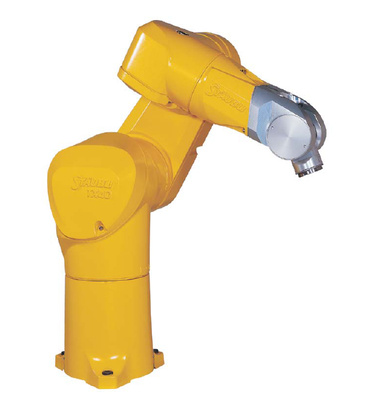
\includegraphics[width=1.5cm]{TX40}\\Stäubli TX40};
		
		\node[block, left = 2cm of TX40](CS8){Robot Control\\Stäubli CS 8};
		
		\coordinate (camPos) at (-4cm, 2.8cm);
		
		
		
		\node[block, fill=white, above left = 1cm and 7cm of TX40](ctrl){Setpoint Generation};
		\node[above = 0.2cm of ctrl, visible on=<2->](matlab-descr){MATLAB};
		
		\begin{scope}[on background layer]
		\node[fill=uniSlightblue, fit=(ctrl)(matlab-descr), visible on=<2->](matlab){};
		\end{scope}
		
		\node[block, below = 1.5cm of -(matlab)](TwinCAT){Soft-PLC\\TwinCAT};
		
		\node[block, above = of TX40](material){Soft Material};
		
		
		\node[below=0.2cm of TwinCAT, visible on=<2->](engPClabel){Engineering PC};
		\node[draw=uniSyellow, dashed, fit=(matlab)(TwinCAT)(engPClabel), visible on=<2->](engPCborder){};
		
		\draw[->](camPos)--(camPos-|ctrl.east);
		\camera{(camPos)}{270}{Cam}
		
		\draw[<->](ctrl)--(TwinCAT);
		\draw[<->](TwinCAT)-- node[above]{uniVAL PLC} (CS8);
		\draw[<->](CS8)--(TX40);
		\draw[<->](TX40) -- (material);
		
		
		\end{tikzpicture}
	\end{figure}
	
\end{frame}


\begin{frame}{The General Architecture}

\vspace*{-1cm}

\begin{figure} 
	\centering
	\begin{tikzpicture}% image
	[every node/.append style={align=center}, % align node labels horizontally centered, allows to break text in more lines
	node distance=1cm %standard sistance between nodes
	]
	
	\node[block](TX40){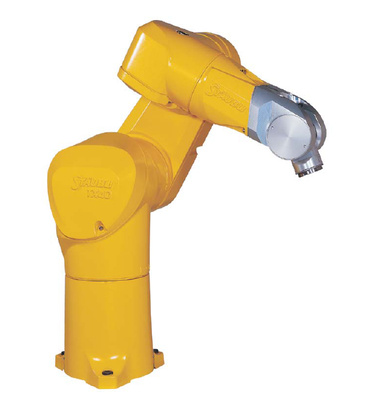
\includegraphics[width=1.5cm]{TX40}\\Stäubli TX40};
	\node[block, right = 4cm of |(TX40)](cable){Cable};
	
	\coordinate (camPos) at (5.7cm, 2.7cm);
	
	\node[block, above = of TX40](imgRec){Image\\Processing};
	\node[block, above = of TX40, fill=uniSlightblue, visible on=<2->](imgRec-highlighted){Image\\Processing};	
	
	\node[block, left = 4cm of imgRec](id){Geometry\\Estimation};
	\node[block, left = 4cm of TX40](ctrl){Model-based\\Control};
	
	\draw[->](TX40) -- node[above]{$\bmat{x & y & \theta_z}^\mathrm{T}$} (cable);
	
	\draw[->](camPos)-- node[above]{Picture \( \bm P \in \R^{1920 \times 1080} \)} (camPos-|imgRec.east);
	\draw[->](imgRec) -- node[above]{Features \(\bm{\hat x} \in \R^{2 \times N} \)} (id);
	\draw[->](id) -- node[right]{$\bm{\hat a},\,L$} (id|-ctrl.north);
	\draw[->](ctrl) -- node[above]{$\bmat{x_\mathrm{des} & y_\mathrm{des} & \theta_{z,\mathrm{des}} }^\mathrm{T}$} (TX40);
	
	\camera{(camPos)}{180}{USB\\Webcam}
	
	\node[below = 0.5cm of TX40, text=uniSlightblue, visible on=<1-1>](twinLabel){Digital Twin};
	\node[dashed, draw=uniSlightblue, fit=(twinLabel)(id)(cable)(ctrl), inner sep=0.3cm, visible on=<1-1>](digitalTwinBorder){};
	
	\node[ellipse, draw, uniSred,minimum width=2cm, minimum height=0.3cm, visible on=<1-1>] (commCircle) at ($(ctrl.east)+(2cm,0)$){};
	\draw[draw=uniSred, visible on=<1-1>](commCircle) |- node[pos=1, left, text=uniSred]{Communication} ++(-1cm, -2cm);
	\end{tikzpicture}
\end{figure}

\end{frame}


% ----------------------------------------------------------------------------------------------------------
%\begin{frame}{Image Processing}
%\begin{itemize}
%\item Depth information of Kinect (RGB-D) not accurate enough  
%\item Problem is modeled 2-dimensional
%\item Chose Webcam (RGB) for better image quality and robust interface
%\item Camera set up at the top of the robot chamber
%\item Intrinsic and extrinsic calibration of camera using a 'checkerboard' 
%
%% \iffalse
%% \begin{itemize}
%% \item Acquire picture
%% \item ROI
%% \item Color: Conversion
%% \item Color: Separation
%% \item Segmentation: Thin out and fill gaps
%% \item Reduce to one pixel per column
%% \item ImageSpace to CoordinateSpace
%% \item Pixel to mm
%% \end{itemize}
%% \fi
%\end{itemize}
%
%\visible<2->{
%\begin{center}
%\begin{quotation}
%"There's a  toolbox for that.."
%\end{quotation}
%\end{center}
%}
%\begin{figure}
%	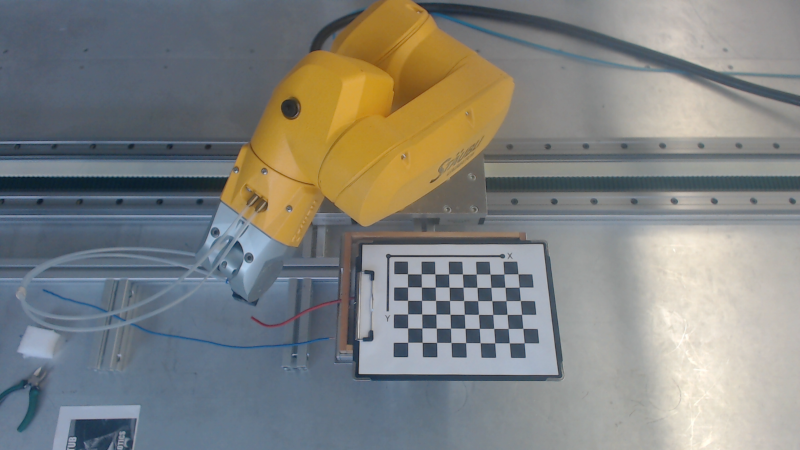
\includegraphics[width=0.35\textwidth]{Checker}
%	\caption{Camera calibration}
%\end{figure}
%
%\end{frame}
\begin{frame}{Image Processing: Pipeline}


\vspace*{-1cm}

\begin{figure} 
	\centering
	\begin{tikzpicture}% image
	[every node/.append style={align=center}, % align node labels horizontally centered, allows to break text in more lines
	node distance=1cm %standard sistance between nodes
	]
	
	\node[block](RGB){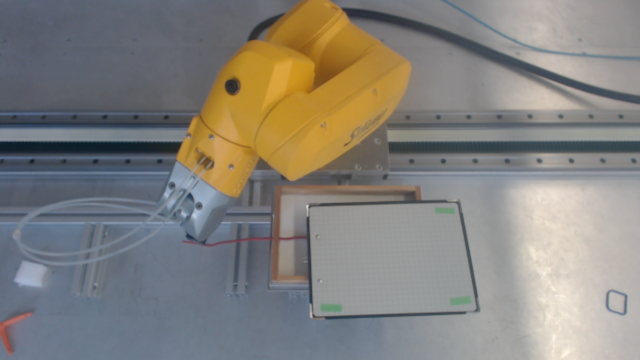
\includegraphics[width=2cm]{Low}\\RGB frame};
    \node[block, right = 1.8cm of |(RGB)](ROI){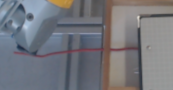
\includegraphics[width=2cm]{ROI_2}\\cropped RGB frame};
	\node[block, right = 1.8cm of |(ROI)](HSV){HSV frame};
    \node[block, right = 1.8cm of |(HSV)](ColBW){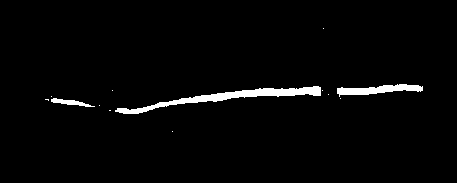
\includegraphics[width=2cm]{ROI_BW}\\BW mask};
	\node[block, below = 1.8cm of |(RGB)](SegBW){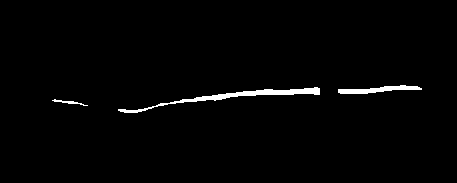
\includegraphics[width=2cm]{ROI_BW_Seg}\\Smoothed mask};
    \node[block, right = 1.8cm of |(SegBW)](ThinBW){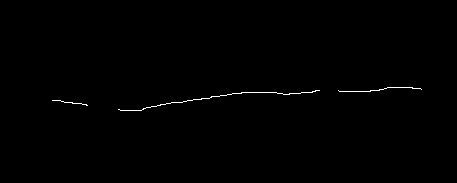
\includegraphics[width=2cm]{ROI_BW_Thin}\\Thinned out mask};
    \node[block, right = 1.8cm of |(ThinBW)](CooSpace){$\bmat{x_{i,1}, x_{i,2}, ...}$\\ Coordinates};
    \node[block, right = 1.8cm of |(CooSpace)](WorldSpace){$\bmat{x_{w,1}, x_{w,2}, ...}$\\World\\coordinates};
	
    \draw[->](RGB) -- node[above]{Region of\\Interest} (ROI);
	\draw[->](ROI) -- node[above]{Colour\\conversion} (HSV);
    \draw[->](HSV) -- node[above]{Colour\\thresholding} (ColBW);
    \draw[->](ColBW.south) |- ++(-6,-1)  node[above]{Erode \& \\dilate} -|(SegBW.north);
    \draw[->](SegBW) -- node[above]{1 pixel per\\column} (ThinBW);
    \draw[->](ThinBW) -- node[above]{Find white\\pixels} (CooSpace);
    \draw[->](CooSpace) -- node[above]{Trans-\\formation} (WorldSpace);
    
    
	%\coordinate (RGB) at (0cm, 0cm);
	
	
	
	%\node[block, above = of TX40](imgRec){Image\\Processing};
	%\node[block, left = 4cm of imgRec](id){Geometry\\Estimation};
	%\node[block, left = 4cm of TX40](ctrl){Model-based\\Control};
	
	
	%\draw[->](camPos)-- node[above]{RGB-Frame} (camPos-|imgRec.east);
	%\draw[->](imgRec) -- node[above]{Features} (id);
	%\draw[->](id) -- node[right]{$\bm{\hat a}$} (id|-ctrl.north);
	%\draw[->](ctrl) -- node[above]{$\bmat{x_\mathrm{des} & y_\mathrm{des} & \theta_{z,\mathrm{des}} }^\mathrm{T}$} (TX40);
	
	%\camera{(camPos)}{180}{USB\\Webcam}
	
	%\node[below = 0.5cm of TX40, text=uniSlightblue](twinLabel){Digital Twin};
	%\node[dashed, draw=uniSlightblue, fit=(twinLabel)(id)(cable)(ctrl), inner sep=0.3cm](digitalTwinBorder){};
	
	%\node[ellipse, draw, uniSred,minimum width=2cm, minimum height=0.3cm] (commCircle) at ($(ctrl.east)+(2cm,0)$){};
	%\draw[draw=uniSred](commCircle) |- node[pos=1, left, text=uniSred]{Communication} ++(-1cm, -2cm);
	\end{tikzpicture}
\end{figure}
\end{frame}

% overview slide:


\begin{frame}{Architecture Overview}

\vspace*{-1cm}

\begin{figure} 
	\centering
	\begin{tikzpicture}% image
	[every node/.append style={align=center}, % align node labels horizontally centered, allows to break text in more lines
	node distance=1cm %standard sistance between nodes
	]
	
	\node[block](TX40){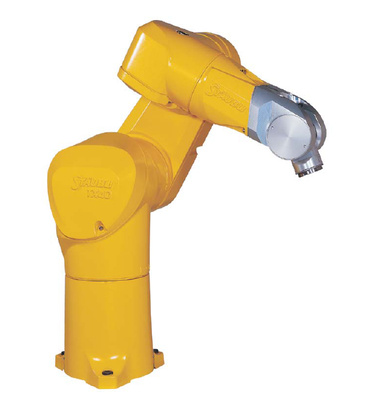
\includegraphics[width=1.5cm]{TX40}\\Stäubli TX40};
	\node[block, right = 4cm of |(TX40)](cable){Cable};
	
	\coordinate (camPos) at (5.7cm, 2.7cm);
	
	
	
	\node[block, above = of TX40](imgRec){Image\\Processing};
	\node[block, left = 4cm of imgRec](id){Geometry\\Estimation};
	\node[block, left = 4cm of TX40](ctrl){Model-based\\Control};
	
	\node[block, above = of TX40, fill=uniSlightblue, visible on=<1-1>](imgRec-highlighted){Image\\Processing};
	\node[block, left = 4cm of imgRec, fill=uniSlightblue, visible on=<2->](id-highlighted){Geometry\\Estimation};
	
	\draw[->](TX40) -- node[above]{$\bmat{x & y & \theta_z}^\mathrm{T}$} (cable);
	
	\draw[->](camPos)-- node[above]{Picture \( \bm P \in \R^{1920 \times 1080} \)} (camPos-|imgRec.east);
	\draw[->](imgRec) -- node[above]{Features \(\bm{\hat x} \in \R^{2 \times N} \)} (id);
	\draw[->](id) -- node[right]{$\bm{\hat a},\,L$} (id|-ctrl.north);
	\draw[->](ctrl) -- node[above]{$\bmat{x_\mathrm{des} & y_\mathrm{des} & \theta_{z,\mathrm{des}} }^\mathrm{T}$} (TX40);
	
	\camera{(camPos)}{180}{USB\\Webcam}
	
	%\node[below = 0.5cm of TX40, text=uniSlightblue](twinLabel){Digital Twin};
	%\node[dashed, draw=uniSlightblue, fit=(twinLabel)(id)(cable)(ctrl), inner sep=0.3cm](digitalTwinBorder){};
	
	%\node[ellipse, draw, uniSred,minimum width=2cm, minimum height=0.3cm, visible on=<2->] (commCircle) at ($(ctrl.east)+(2cm,0)$){};
	%\draw[draw=uniSred, , visible on=<2->](commCircle) |- node[pos=1, left, text=uniSred, visible on=<2->]{Communication} ++(-1cm, -2cm);
	\end{tikzpicture}
\end{figure}

\end{frame}

% ---------------------------------------------------------------------------------------------------------
\begin{frame}{Geometry Estimation}

\begin{columns}
	\begin{column}{.6\textwidth}
%		\structure{Description of the cable}
		\begin{itemize}
			\item Description by curvature angle $\theta$:
			\begin{equation*}
			\begin{array}{lll}
			\textbf{x}(s,t) =\textbf{x}(0,t)+ \displaystyle\int\limits_0^s
			\left[
			\begin{array}{ll}
			\mathrm{cos}\big(\theta(u)\big) \\
			\mathrm{sin}\big(\theta(u)\big)
			\end{array}
			\right]
			\,\mathrm{d}u
			\end{array}
			\end{equation*}
			\item Formulate a optimization problem
			  \begin{equation*}
			\begin{array}{lll}
			F(\hat{\textbf{a}},L,\hat{\textbf{s}}) =& \sum\limits_{j=1}^{N} \Vert \textbf{x}(\bar{s}_i) - \hat{\textbf{x}}_j \Vert_2^2   \quad &\ldots\text{ fit to data}\\[4mm]
			&+ \alpha_1\, \sum\limits_{i=2}^{n} a_i^2     \quad &\ldots\text{ regularization}\\[4mm]
			&+ \alpha_2\, (L - L_\text{expected})^2         \quad &\ldots\text{ avoid overfitting}\\[4mm]
			&+ \alpha_3\, \Vert \textbf{x}(L) - \textbf{x}_\text{end}\Vert_2^2    \quad &\ldots\text{ ensure end point}\\[4mm]
			\end{array}
			\end{equation*} 
			
			%$f_{0, \mathrm{triv}} = \min \quad \|\bm x(s_i) - \hat{\bm x}_i\|^2$
		\end{itemize}
	\end{column}

	\begin{column}{.4\textwidth}
		\includegraphics[width=\columnwidth]{model.eps}
		\begin{flushright}
			{\tiny	\textcolor{uniSgrey!50}{ Source: \cite{wakamatsu2004}} } 
		\end{flushright}
	\end{column}
\end{columns}


\end{frame}

% ----------------------------------------------------------------------------------------------------------
%\begin{frame}{Geometry Estimation}
%\begin{itemize}
%\item The $n$ ansatz functions, $e_i(u)$, are given by
%\begin{equation*}
%  \begin{array}{lll}
%    e_0(s) = 1, \quad e_1(s) = s/L, \\[4mm]
%    e_{2i+1}(s) = \mathrm{sin}(2\pi i s)/L, \quad e_{2i+2}(s) = \mathrm{cos}(2\pi i s)/L \quad i=1,2,3,4,\ldots,
%  \end{array}
%\end{equation*}
%where $L$ is the length of the curve (Similar to \cite{wakamatsu2004}).
%\begin{figure}
%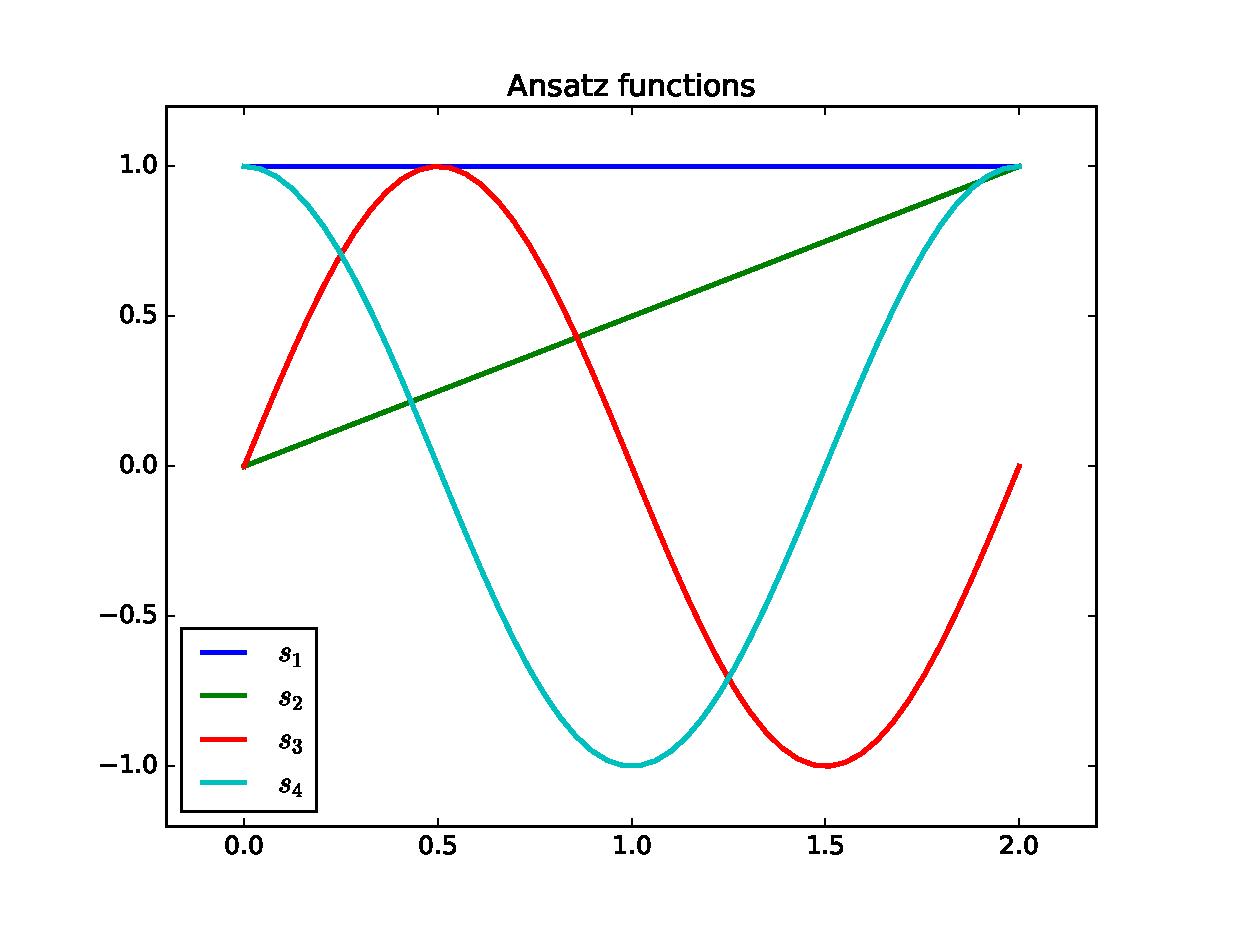
\includegraphics[width=0.4\textwidth]{img/ansatz_functions.eps}
%\caption{Ansatz functions $e_i, i=1,\dots,4$}
%\end{figure}
%\end{itemize}
%
%\end{frame}

% ----------------------------------------------------------------------------------------------------------
%\begin{frame}{Geometry Estimation}
%\structure{Determining the curve parameters $a_i$, $L$:}
%\begin{itemize}
%  \item Reduce input point cloud $\{\hat{\textbf{x}}_j\}_{j=1}^{N_p}$ to $N$ points $\{\hat{\textbf{x}}_j\}_{j=1}^{N}$ by taking every $N_p/N$-th point.
%  \item Minimize the following nonlinear least-squares objective function:
%  \begin{equation*}
%    \begin{array}{lll}
%      F(\hat{\textbf{a}},L,\hat{\textbf{s}}) =& \sum\limits_{j=1}^{N} \Vert \textbf{x}(\bar{s}_i) - \hat{\textbf{x}}_j \Vert_2^2   \quad &\ldots\text{ fit to data}\\[4mm]
%        &+ \alpha_1\, \sum\limits_{i=2}^{n} a_i^2     \quad &\ldots\text{ regularization}\\[4mm]
%        &+ \alpha_2\, (L - L_\text{expected})^2         \quad &\ldots\text{ avoid overfitting}\\[4mm]
%        &+ \alpha_3\, \Vert \textbf{x}(L) - \textbf{x}_\text{end}\Vert_2^2    \quad &\ldots\text{ ensure end point}\\[4mm]
%    \end{array}
%  \end{equation*}
%\end{itemize}
%
%\end{frame}


\begin{frame}{Architecture Overview}

\vspace*{-1cm}

\begin{figure} 
	\centering
	\begin{tikzpicture}% image
	[every node/.append style={align=center}, % align node labels horizontally centered, allows to break text in more lines
	node distance=1cm %standard sistance between nodes
	]
	
	\node[block](TX40){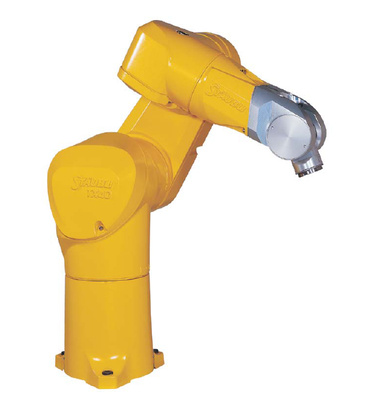
\includegraphics[width=1.5cm]{TX40}\\Stäubli TX40};
	\node[block, right = 4cm of |(TX40)](cable){Cable};
	
	\coordinate (camPos) at (5.7cm, 2.7cm);
	
	
	
	\node[block, above = of TX40](imgRec){Image\\Processing};
	\node[block, left = 4cm of imgRec](id){Geometry\\Estimation};
	\node[block, left = 4cm of TX40](ctrl){Model-based\\Control};
	
	\node[block, left = 4cm of imgRec, fill=uniSlightblue, visible on=<1-1>](id-highlighted){Geometry\\Estimation};
	\node[block, left = 4cm of TX40, fill=uniSlightblue, visible on=<2->](ctrl-highlighted){Model-based\\Control};
	
	\draw[->](TX40) -- node[above]{$\bmat{x & y & \theta_z}^\mathrm{T}$} (cable);
	
	\draw[->](camPos)-- node[above]{Picture \( \bm P \in \R^{1920 \times 1080} \)} (camPos-|imgRec.east);
	\draw[->](imgRec) -- node[above]{Features \(\bm{\hat x} \in \R^{2 \times N} \)} (id);
	\draw[->](id) -- node[right]{$\bm{\hat a},\,L$} (id|-ctrl.north);
	\draw[->](ctrl) -- node[above]{$\bmat{x_\mathrm{des} & y_\mathrm{des} & \theta_{z,\mathrm{des}} }^\mathrm{T}$} (TX40);
	
	\camera{(camPos)}{180}{USB\\Webcam}
	
	%\node[below = 0.5cm of TX40, text=uniSlightblue](twinLabel){Digital Twin};
	%\node[dashed, draw=uniSlightblue, fit=(twinLabel)(id)(cable)(ctrl), inner sep=0.3cm](digitalTwinBorder){};
	
	%\node[ellipse, draw, uniSred,minimum width=2cm, minimum height=0.3cm, visible on=<2->] (commCircle) at ($(ctrl.east)+(2cm,0)$){};
	%\draw[draw=uniSred, , visible on=<2->](commCircle) |- node[pos=1, left, text=uniSred, visible on=<2->]{Communication} ++(-1cm, -2cm);
	\end{tikzpicture}
\end{figure}

\end{frame}


%====================================================================
% ----------------------------------------------------------------------------------------------------------
%===================================================================
%\begin{frame}{Model based Control - Model}
%\centering
%\includegraphics[width=.65\columnwidth]{model.eps}
%\begin{flushright}
%	{\tiny	\textcolor{uniSgrey!50}{ Source: \cite{wakamatsu2004}} }
%\end{flushright}

%\includegraphics[scale=0.5]{Plots/model}
%\end{frame}

%\begin{frame}{Model based Control - Model}
%\begin{itemize}
%%\item \textbf{Picture}: line, gripper, heavy object at end
%\item Kinetic Energy:
%\begin{align*}
%T=&\dfrac{1}{2}\int_0^L \rho v^2(s,t) ds+\dfrac{1}{2}m_Lv^2(L,t)+\dfrac{1}{2}J_L\dot{\theta}^2(L,t)
%\end{align*}
%\item Potential Energy
%\begin{align*}
%U=&\dfrac{1}{2}\int_0^L R_{flex} \left(\dfrac{d\theta}{ds}\right)^2ds%=
%%U=&\dfrac{1}{2}\int_0^L R_{flex}\sum_{i=1}^n\sum_{j=1}^n \dfrac{\partial e_i}{\partial s}\dfrac{\partial e_j}{\partial s}a_ia_j ds\\
%%=&\dfrac{1}{2}\sum_{i=1}^n\sum_{j=1}^n K_{ij}a_ia_j=\dfrac{1}{2}a^\top K a
%\end{align*}
%\item Lagrangian $L=T-U$: modal dynamic
%\begin{align*}
%\dfrac{d}{dt}\dfrac{\partial L}{\partial \dot{a}_i}-\dfrac{\partial L}{\partial a_i}=0
%\end{align*}
%\item \textbf{Simplification}: assume steady-state\quad 
%  $\dot{x}_0=\dot{y}_0=\dot{\theta}_0=\dot{a}_j\approx 0$.
%%\begin{align*}%
%%\dfrac{d}{dt}\left(\dfrac{\partial T}%{\dot{a}_i}\right)=&\ddot{x}_0\overline{S}_i+\ddot{y}_0\overline{C}_i+\ddot{\theta}_0m_{%0i}+\sum_{j=1}^n m_{ij}\ddot{a}_j\\
%%&+m_L((\ddot{x}_0+\ddot{\theta}_0S_0)S_i+%(\ddot{y}_0+\ddot{\theta}_0C_0)C_i+\sum_{j=1}^n[S_iS_j+C_iC_j]_{s=L}\ddot{a}_j\\
%%&+J_L(\ddot{\theta}_0e_i(L)+\sum_{j=1}^n e_i(L)e_j(L)\ddot{a}_j)
%%\end{align*}
%%Vector:
%\begin{align*}
%M\ddot{a}+Ka+B_1\ddot{x}_0+B_2\ddot{y}_0+B_3\ddot{\theta}_0=0\quad 
%M_{ij}=\int_0^L\rho [S_iS_j+C_iC_j]ds+\dots
%%M\ddot{a}+Ka+\tilde{B}u=0\\
%\end{align*}
%\item First-order model:
%\begin{align*}
%\dot{x}=Ax+Bu,\quad x=[a,\dot{a}],\quad u=[\ddot{x}_0,\ddot{y}_0,\ddot{\theta}_0].
%\end{align*}
%\end{itemize}
%\footnotetext{Dynamic Modeling of Linear Object Deformation based on Differential Geometry Coordinates \cite{wakamatsu2005dynamic}}
%\end{frame}


% ----------------------------------------------------------------------------------------------------------
\begin{frame}{Model based Control - Control algorithm}
\large{\textbf{Two options}}
\normalsize
\begin{itemize}
\item \textbf{Linear quadratic regulator} (LQR)\\
\vspace{1mm}
objective functional: $\min_u\int_0^\infty \|x\|_Q^2+\|u\|_R^2 d\tau$\\
\vspace{1mm}
experienced some technical/numerical issues 
\vspace{3mm}
\item \textbf{Predictive (functional) control}
\begin{enumerate}
\vspace{1mm}
\item Transform model: acceleration $u$ $\stackrel{a_{\max},v_{\max},T_s}{\Leftrightarrow}$ relative position command to robot
\vspace{1mm}
\item Formulate objective function: 
\begin{align*}
\min_{u\in\mathbb{U}}&\|y(L)-y_{ref}\|^2+\|u\|^2\\
\text{s.t. }&\Delta a=B_d u,\quad \theta(s)=\sum_i a_ie_i(s)
\quad  y(L)=\int_0^L \cos(\theta(s))ds,\quad %&u\in\mathcal{U}
\end{align*}
\vspace{1mm}
\item use CasADi to solve optimization problem online (for a given configuration $a$)
\vspace{1mm}
\item Give position command with maximal velocity/acceleration to robot control 
\end{enumerate}
\end{itemize}
\end{frame}
%====================================================================
% ----------------------------------------------------------------------------------------------------------
%====================================================================

\begin{frame}{Architecture Overview}

\vspace*{-1cm}

\begin{figure} 
	\centering
	\begin{tikzpicture}% image
	[every node/.append style={align=center}, % align node labels horizontally centered, allows to break text in more lines
	node distance=1cm %standard sistance between nodes
	]
	
	\node[block](TX40){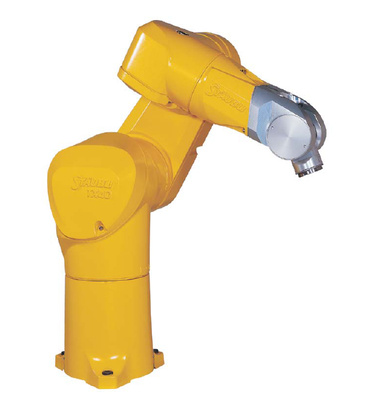
\includegraphics[width=1.5cm]{TX40}\\Stäubli TX40};
	\node[block, right = 4cm of |(TX40)](cable){Cable};
	
	\coordinate (camPos) at (5.7cm, 2.7cm);
	
	
	
	\node[block, above = of TX40](imgRec){Image\\Processing};
	\node[block, left = 4cm of imgRec](id){Geometry\\Estimation};
	\node[block, left = 4cm of TX40](ctrl){Model-based\\Control};
	
	\node[block, left = 4cm of TX40, fill=uniSlightblue, visible on=<1-1>](ctrl-highlighted){Model-based\\Control};
	
	\draw[->](TX40) -- node[above]{$\bmat{x & y & \theta_z}^\mathrm{T}$} (cable);
	
	\draw[->](camPos)-- node[above]{Picture \( \bm P \in \R^{1920 \times 1080} \)} (camPos-|imgRec.east);
	\draw[->](imgRec) -- node[above]{Features \(\bm{\hat x} \in \R^{2 \times N} \)} (id);
	\draw[->](id) -- node[right]{$\bm{\hat a},\,L$} (id|-ctrl.north);
	\draw[->](ctrl) -- node[above]{$\bmat{x_\mathrm{des} & y_\mathrm{des} & \theta_{z,\mathrm{des}} }^\mathrm{T}$} (TX40);
	
	\camera{(camPos)}{180}{USB\\Webcam}
	
	%\node[below = 0.5cm of TX40, text=uniSlightblue](twinLabel){Digital Twin};
	%\node[dashed, draw=uniSlightblue, fit=(twinLabel)(id)(cable)(ctrl), inner sep=0.3cm](digitalTwinBorder){};
	
	\node[ellipse, draw, uniSred,minimum width=2cm, minimum height=0.3cm, visible on=<2->] (commCircle) at ($(ctrl.east)+(2cm,0)$){};
	\draw[draw=uniSred, , visible on=<2->](commCircle) |- node[pos=1, left, text=uniSred, visible on=<2->]{Communication} ++(-1cm, -2cm);
	\end{tikzpicture}
\end{figure}

\end{frame}

%\begin{frame}{Communication}
%
%\vspace*{-1cm}
%
%\begin{columns}
%	\begin{column}{.5\textwidth}
%		\structure{Problems:}
%		\begin{itemize}
%			\item TwinCAT cycle time (milliseconds) vs. image recognition (some seconds)
%			\onslide<2->{\item uniVAL PLC interface only provides final target points with velocity and acceleration percentage of \emph{nominal values}, control requires \(a_\mathrm{des}(t)\)}
%		\end{itemize}
%		\onslide<3->{
%		\structure{Key question:}
%		\begin{itemize}
%			\item How to communicate between MATLAB controller and TwinCAT? \pause
%			\begin{itemize}
%				\item TwinCAT Simulink interface
%				\item Direct network communication
%			\end{itemize}
%		\end{itemize} 
%		} % end onslide <3->
%	\end{column}
%	\begin{column}{.5\textwidth}
%		\onslide<2->{
%		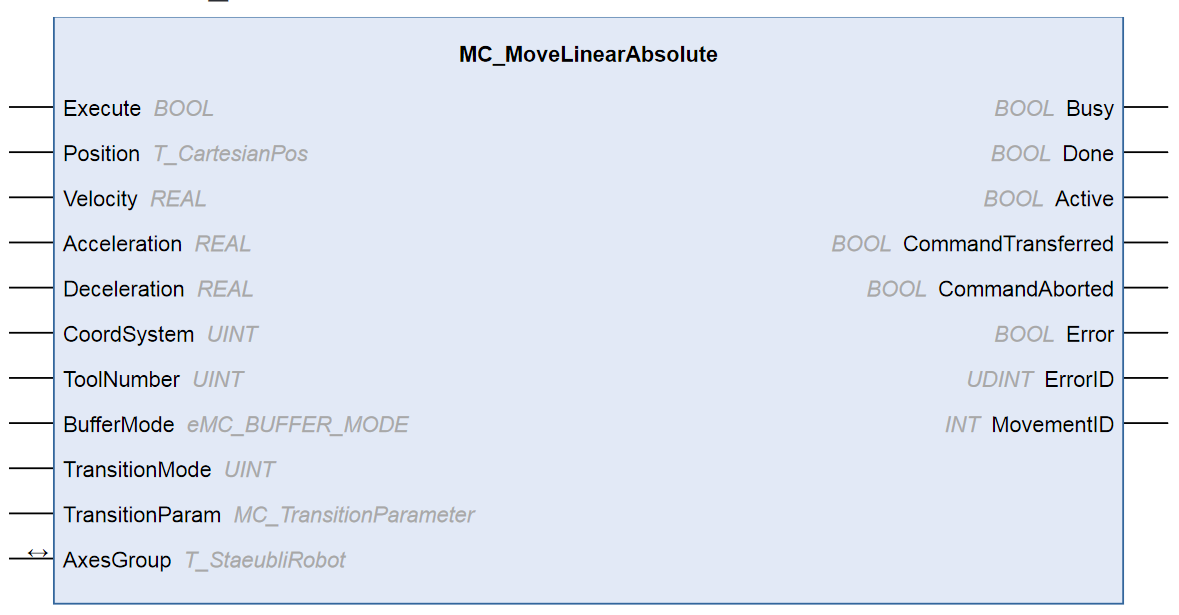
\includegraphics[width=\columnwidth]{MC_MoveLinearAbsolute}
%		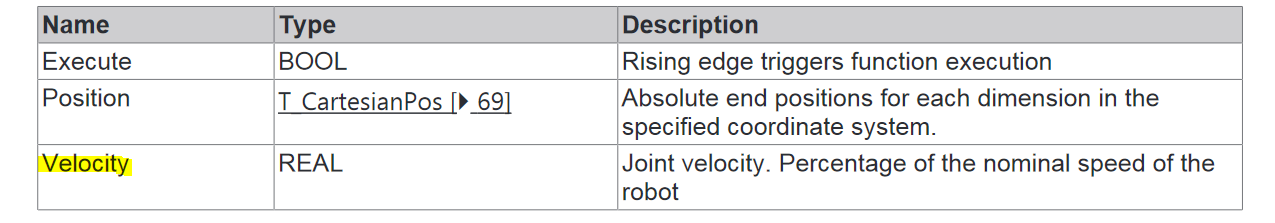
\includegraphics[width=\columnwidth]{VelCommandUniVAL}
%		} % end onslide<2->
%	\end{column}
%\end{columns}
%
%\end{frame}

\begin{frame}{Communication -- Sequence and Protocol}
%
%\centering
%
%%\begin{tikzpicture}
%%\begin{umlseqdiag}
%%	\umlobject[no ddots]{Stäubli RC}
%%	\umlobject[no ddots,x=2.5]{PLC RC}
%%	\umlobject[no ddots, x=6]{PLC communication}
%%	\umlobject[no ddots, x=9.5]{MATLAB control}
%%	
%%	\begin{umlfragment}[type=loop, label=forever, inner xsep=4]
%%	
%%	\begin{umlcall}[op={getSetpoint(TCP pose)}, return={desired TCP pose}, dt=8]{PLC RC}{PLC communication}
%%	\begin{umlcall}[op={getSetpoint(TCP pose)}, return={desired TCP pose}]{PLC communication}{MATLAB control}
%%	\begin{umlcallself}[op=getSetpoint()]{MATLAB control}
%%	\end{umlcallself}
%%	\end{umlcall}
%%	
%%	\end{umlcall}
%%	
%%	\begin{umlcall}[op=moveLinear(), return=hasFinished]{PLC RC}{Stäubli RC}
%%	\end{umlcall}
%%	
%%	\end{umlfragment}
%%	
%%\end{umlseqdiag}
%\end{tikzpicture}


\begin{itemize}
	\item Communication between MATLAB and Stäubli RC over Matlab \(\leftrightarrow\) TwinCAT \(\leftrightarrow\) Stäubli RC 
	\item No real-time  communication
	\item Only open loop control of setpoints
\end{itemize}

\end{frame}



% Digital Twin Overview:
\begin{frame}{Architecture Overview}

\vspace*{-1cm}

\begin{figure} 
	\centering
	\begin{tikzpicture}% image
	[every node/.append style={align=center}, % align node labels horizontally centered, allows to break text in more lines
	node distance=1cm %standard sistance between nodes
	]
	
	\node[block](TX40){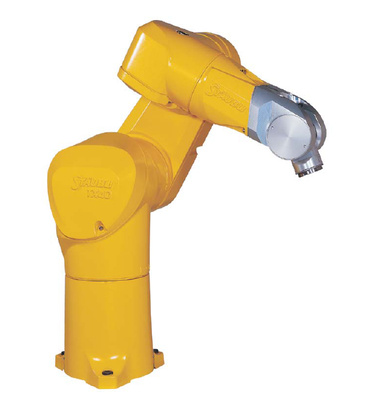
\includegraphics[width=1.5cm]{TX40}\\Stäubli TX40};
	\node[block, right = 4cm of |(TX40)](cable){Cable};
	
	\coordinate (camPos) at (5.7cm, 2.7cm);
	
	
	
	\node[block, above = of TX40](imgRec){Image\\Processing};
	\node[block, left = 4cm of imgRec](id){Geometry\\Estimation};
	\node[block, left = 4cm of TX40](ctrl){Model-based\\Control};
	
	\draw[->](TX40) -- node[above]{$\bmat{x & y & \theta_z}^\mathrm{T}$} (cable);
	
	\draw[->](camPos)-- node[above]{Picture \( \bm P \in \R^{1920 \times 1080} \)} (camPos-|imgRec.east);
	\draw[->](imgRec) -- node[above]{Features \(\bm{\hat x} \in \R^{2 \times N} \)} (id);
	\draw[->](id) -- node[right]{$\bm{\hat a},\,L$} (id|-ctrl.north);
	\draw[->](ctrl) -- node[above]{$\bmat{x_\mathrm{des} & y_\mathrm{des} & \theta_{z,\mathrm{des}} }^\mathrm{T}$} (TX40);
	
	\camera{(camPos)}{180}{USB\\Webcam}
	
	\node[below = 0.5cm of TX40, visible on=<2->](twinLabel){Digital Twin};
	\begin{scope}[on background layer]
	\node[fill=uniSlightblue, fit=(twinLabel)(id)(cable)(ctrl), inner sep=0.3cm, visible on=<2->](digitalTwinBorder){};
	\end{scope}
	%\node[ellipse, draw, uniSred,minimum width=2cm, minimum height=0.3cm, visible on=<2->] (commCircle) at ($(ctrl.east)+(2cm,0)$){};
	%\draw[draw=uniSred, , visible on=<2->](commCircle) |- node[pos=1, left, text=uniSred, visible on=<2->]{Communication} ++(-1cm, -2cm);
	\end{tikzpicture}
\end{figure}

\end{frame}


% ----------------------------------------------------------------------------------------------------------
\begin{frame}{Digital Twin}

\vspace*{-1cm}
\begin{columns}
	\begin{column}{.5\textwidth}
		\structure{Robot simulation:}
		\begin{itemize}
			\item Realtime simulation Tool ISG-virtuos
			\item Kinematic model of the ABB IRB 1600
 		\end{itemize}
        \structure{Cable simulation:}
        \begin{itemize}
			\item Physics engine AGX-Algoryx
            \item Multi-(Rigid)-body model
			\item Integration into ISG-virtuos as an FMU (FMI-Interface Standard)
 		\end{itemize}
        \structure{Virtual Robot Control:}
        \begin{itemize}
			\item CNC Kernel with inverse kinematics
			\item Integrated into Robot simulation environment
 		\end{itemize}
        \structure{Virtual Camera (not realized):}
        \begin{itemize}
			\item Direct feature output out of the cable model
 		\end{itemize}
        \end{column}
     \begin{column}{.5\textwidth}
     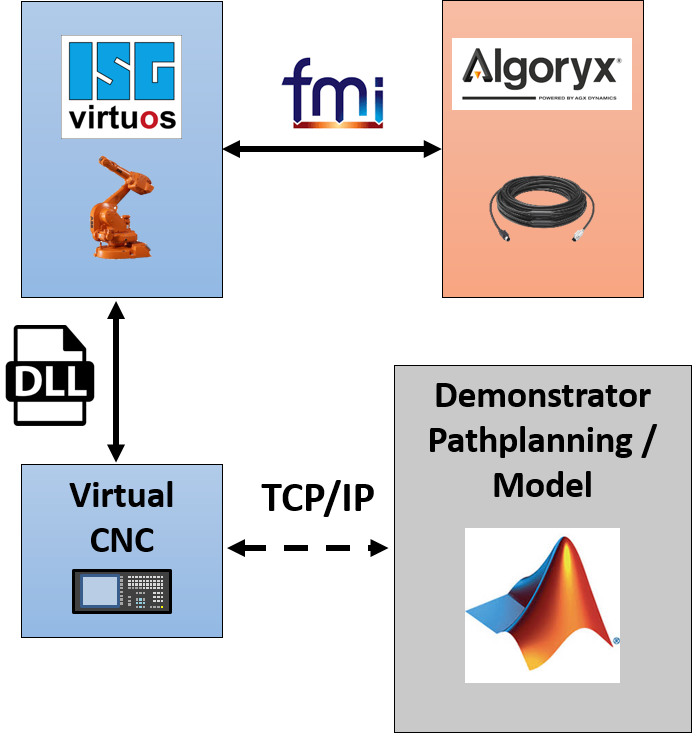
\includegraphics[width=.8\columnwidth]{Digital_Twin}
     \end{column}
       
\end{columns}
\end{frame}


% ----------------------------------------------------------------------------------------------------------

% ----------------------------------------------------------------------------------------------------------
\section{Results}

\begin{frame}{Digital Twin}
	\begin{center}		
		\movie[width=0.8\linewidth,
		height=0.45\linewidth,poster]{}{vid/DigitalTwin_shorted.mov}
		
		%		\includemedia[
		%		width=0.6\linewidth,
		%		height=0.5\linewidth,
		%		activate=pageopen,
		%		addresource=vid/ABB_Kabel2.MP4,
		%		flashvars={source=vid/ABB_Kabel2.MP4}
		%		]{}{VPlayer.swf}
	\end{center}
\end{frame}

\begin{frame}{Real Scenario}
	\begin{center}
		
		\movie[width=0.8\linewidth,
		height=0.45\linewidth,poster]{}{vid/ResultVideo.mov}
		
%		\includemedia[
%			width=0.6\linewidth,
%			height=0.5\linewidth,
%			activate=pageopen,
%			addresource=vid/SummerSchool2018_CablePositionControl.MP4,
%			flashvars={source=vid/SummerSchool2018_CablePositionControl.MP4}
%			]{}{VPlayer.swf}
	\end{center}	

\end{frame}

% ----------------------------------------------------------------------------------------------------------
\section{Conclusion}

\begin{frame}{Conclusion \& next steps}


	\begin{columns}
	\begin{column}{0.5\textwidth}
	\structure{Proof of concept}
		\begin{itemize}
			\item Based on visual data acquisition and processing
			\item Model based position control
			\item Toolchain for position control over TCP/IP
		\end{itemize}
	\structure{Possible extensions}
	\begin{itemize}
		\item Identified and experienced problems of the overall toolchain
		\item Recognizing the complexity of the problem and challenges to overcome
	\end{itemize}
	\end{column}
	\begin{column}{0.5\textwidth}
		\begin{center}
			\begin{figure}
				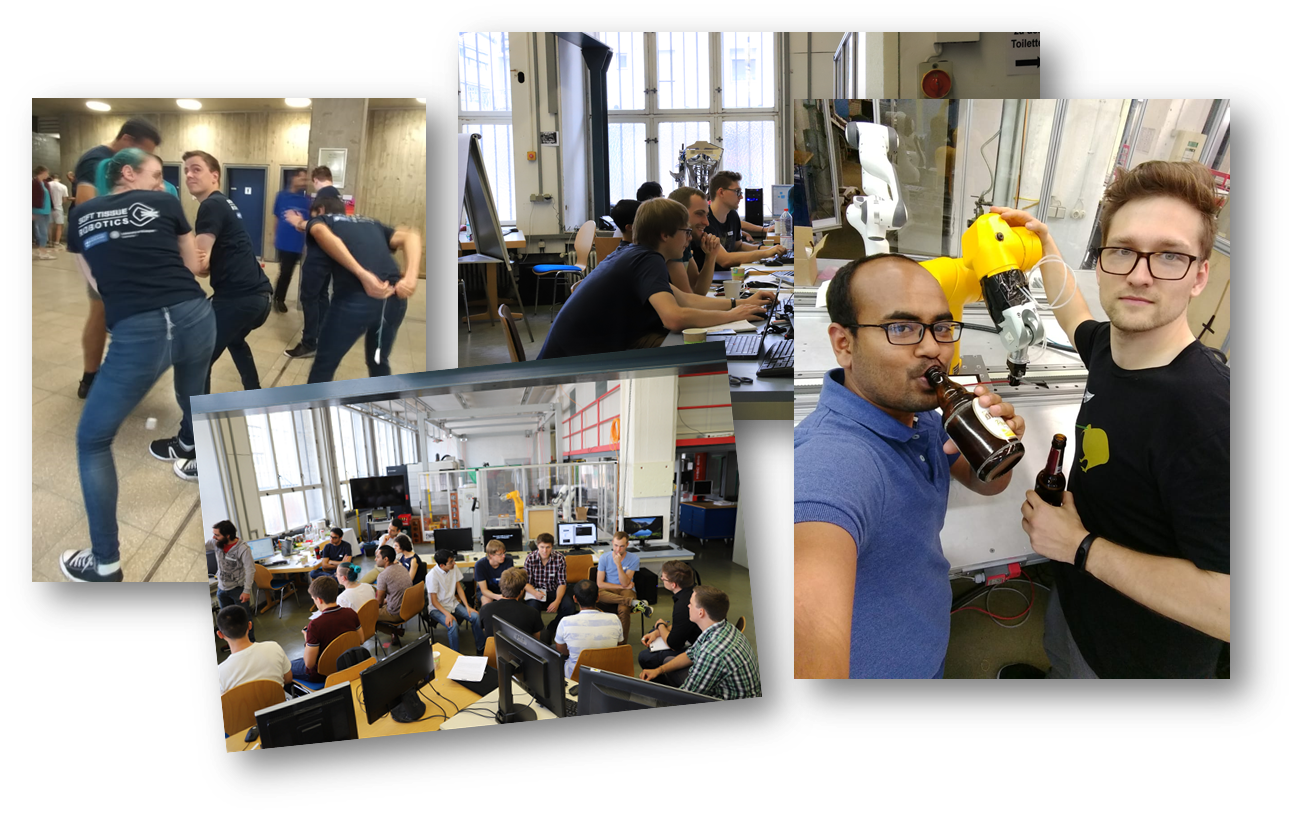
\includegraphics[width=1.1\textwidth]{img/FinalPictureCollage}
			\end{figure}
		\end{center}
	\end{column}
\end{columns}

\end{frame}

% ----------------------------------------------------------------------------------------------------------

\begin{frame}{Literature}
\bibliographystyle{alpha}
%\bibliographystyle{plain}
\bibliography{literature}


\end{frame}



\end{document}
